\documentclass[11pt]{beamer}

\usetheme{Madrid}
\usecolortheme{default}

\title[Pêndulo Simples]{Pêndulo Simples com Newton-Raphson}
\subtitle{Resolvendo o pêndulo simples usando o método de Newton-Raphson}
\author[Gabriel, Pedro e Wiltord]{Gabriel Demba - 15618344\\
Pedro Martins Oliveira - 13696213\\
Wiltord Nyakeruma Mosingi - 15595392}
\institute[ICMC]{Instituto de Ciências Matemáticas e de Computação (ICMC)}
\date[Jun 2026]{Junho 9,2026}

\AtBeginSection[]
{
    \begin{frame}
        \frametitle{Sumário}
        \tableofcontents[currentsection]
    \end{frame}
}

\begin{document}

\begin{frame}
  \titlepage
\end{frame}

\begin{frame}{Sumário}
  \tableofcontents
\end{frame}

\section{Introdução e Contextualização}

\subsection{Pêndulo Simples}

\begin{frame}{Problema do Pêndulo Simples}
    O pêndulo simples é um sistema físico constituído por uma massa pontual presa a uma haste capaz de rotacionar e sob efeito da gravidade.

    \begin{figure}
        \centering
        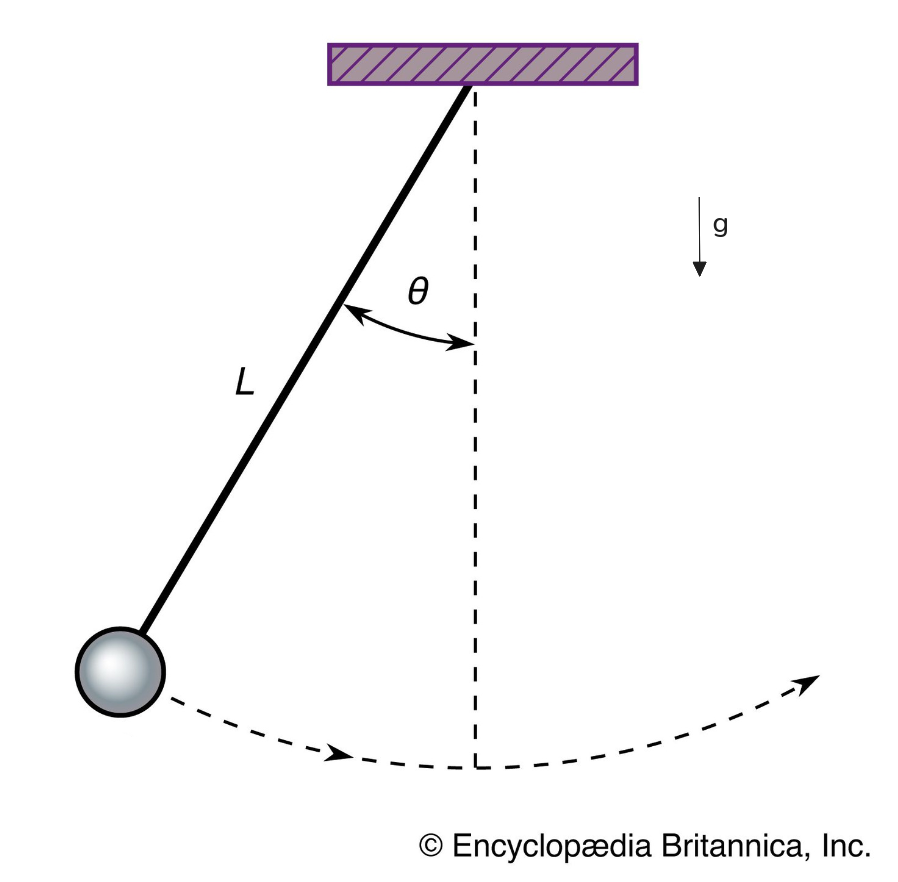
\includegraphics[width=0.3\linewidth]{images/pendulo.png}
        \label{fig:pend}
    \end{figure}

    \pause

    O movimento angular pode ser descrito pela equação \ref{eq:pendulo}:

    \begin{equation}
        \theta''(t) + \frac{g}{L}\sin(\theta(t)) = 0
        \label{eq:pendulo}
    \end{equation}
\end{frame}
% Pra chegar nessa equação só decompor a força gravitacional e igualar com o torque, depois abre o torque e o momento de inércia

\begin{frame}{Problema do Pêndulo Simples}
    Para fugir da não-linearidade, fazemos a aproximação do $\sin(\theta) \approx \theta$ para ângulos pequenos, assim chegamos na equação de um oscilador harmônico \ref{eq:pendulo-aproximado}.

    \begin{equation}
    \begin{split}
        \theta''(t) + \frac{g}{L}\theta(t) &= 0 \\
        \theta(t) &= \theta_0\cos\left( \sqrt{\frac{g}{L}}t \right)
        \label{eq:pendulo-aproximado}
    \end{split}
    \end{equation}

    Para resolver o sistema sem essa aproximação, precisamos utilizar outros métodos
\end{frame}

\begin{frame}{Pêndulo como Problema de Valor de Contorno}
    Podemos encarar o pêndulo simples como um problema diferente se fixarmos um tempo inicial e final $(t\in [0,T])$ e uma posição inicial e final $(\theta(0) = \alpha, \theta(T) = \beta)$ ele se torna um problema de valor de contorno (PVC).

    \vspace{0.4cm}
    \pause

    Para os métodos computacionais também precisamos dividir o tempo (antes contínuo) em passos, usando $m$ passos com intervalo de $h = T/(m+1)$.
\end{frame}

\begin{frame}{Pêndulo como Problema de Valor de Contorno}
    Nessas condições, $\theta(t)$ se torna um vetor $\vec\theta\in\mathbb R^m = (\theta_1, \theta_2, \dots, \theta_m)$, lembrando que o primeiro e o último componente são fixos.
    
    \vspace{0.3cm}
    \pause

    Agora o sistema pode ser descrito como na equação \ref{eq:sistema-raiz}

    \begin{equation}
        G(\vec\theta) = \vec0
        \label{eq:sistema-raiz}
    \end{equation}

    \begin{equation}
        G:\mathbb R^m \to \mathbb R^m = \frac{(\theta_{i-1} - 2\theta_i + \theta_{i+1})}{h^2} + \frac{g}{L}\sin(\theta_i)
    \end{equation}

    $G$ consiste de uma aproximação discreta da segunda derivada da equação original.
\end{frame}

\subsection{Método de Newton-Raphson}

\begin{frame}{Método de Newton-Raphson}
    Usado para encontrar as raízes de equações (lineares ou não), ou seja, para um dado $f:\mathbb R \to \mathbb R$ encontra $x$ tal que $f(x) = 0$.
    
    \vspace{0.4cm}
    
    O método precisa de um chute inicial $x_0$, então ele itera criando novos valores de $x$ seguindo a equação \ref{eq:newton-raphson-iter}.

    \begin{equation}
        x_{i+1} = x_i - \frac{f(x_i)}{f'(x_i)}
        \label{eq:newton-raphson-iter}
    \end{equation}
\end{frame}

\subsection{Algoritmo de Thomas}

\begin{frame}{Algoritmo de Thomas}
    O algoritmo de Thomas é uma forma de resolver sistemas lineares quando a matriz dos coeficientes é tridiagonal, ou seja, os únicos elementos não nulos são os da diagonal principal, da diagonal inferior e da diagonal superior.

    \vspace{0.2cm}

    Nesse algoritmo, não salvamos todos os elementos da matriz visto que a maior parte deles são nulos, salvamos apenas as 3 diagonais.

    \vspace{0.2cm}

    Considere um sistema como na equação \ref{eq:thomas-system}.

    \begin{equation}
        \begin{bmatrix} 
        b_1 & c_1 & 0 & 0 & \cdots & 0 \\ 
        a_2 & b_2 & c_2 & 0 & \cdots & 0 \\ 
        0 & a_3 & b_3 & c_3 & \cdots & 0 \\ 
        \vdots & \vdots & \ddots & \ddots & \ddots & \vdots \\ 
        0 & 0 & \cdots & a_{n-1} & b_{n-1} & c_{n-1} \\ 
        0 & 0 & \cdots & 0 & a_n & b_n 
        \end{bmatrix} 
        \begin{bmatrix} 
        x_1 \\ 
        x_2 \\ 
        x_3 \\ 
        \vdots \\ 
        x_{n-1} \\ 
        x_n 
        \end{bmatrix} 
        = 
        \begin{bmatrix} 
        d_1 \\ 
        d_2 \\ 
        d_3 \\ 
        \vdots \\ 
        d_{n-1} \\ 
        d_n 
        \end{bmatrix}
        \label{eq:thomas-system}
    \end{equation}

\end{frame}

\begin{frame}{Algoritmo de Thomas}
    O algoritmo consiste então de realizar uma eliminação transformando a matriz dos coeficientes numa matriz triangular superior.
    
    \vspace{0.2cm}
    
    Os novos coeficientes são indicados com linha, não precisamos alterar a diagonal principal, usamos as equações \ref{eq:thomas-eliminacao-c} e \ref{eq:thomas-eliminacao-d}.

    \begin{equation}
        c'_i = \Bigg\{\begin{matrix}
            c_i/b_i & i=1 \\[0.1em]
            c_i/(b_i-a_ic'_{i-1}) & \text{outros casos}
        \end{matrix}
        \label{eq:thomas-eliminacao-c}
    \end{equation}
    
    \begin{equation}
        d'_i = \Bigg\{\begin{matrix}
            d_i/b_i & i=1 \\[0.1em]
            (d_i-a_id'_{i-1})/(b_i-a_ic'_{i-1}) & \text{outros casos}
        \end{matrix}
        \label{eq:thomas-eliminacao-d}
    \end{equation}

    Feito isso, basta fazer uma substituição regressiva, da mesma forma que já vimos antes.
\end{frame}

\section{Metodologia}

\subsection{Adaptando Newton-Raphson para sistema de equações}

\begin{frame}{Newton-Raphson para Sistema de Equações}
    O método de newton-raphson é usado para encontrar a raiz de funções, não para sistemas de equações.

    \vspace{0.3cm}

    Logo, vamos adaptar o método da seguinte forma:

    \begin{equation*}
    \begin{split}
        x_{i+1} & = x_i - \frac{f(x_i)}{f'(x_i)} \\
        f'(x_i)\ x_{i+1} & = x_i - f(x_i) \\
        f'(x_i)\ \Delta x & = -f(x_i) \\
        \Delta x & = x_{i+1} - x_i
    \end{split}
    \end{equation*}

\end{frame}

\begin{frame}{Newton-Raphson para Sistema de Equações}
    É importante reforçar que, no contexto de sistema de $n$ equações temos que:

    \begin{table}[]
        \centering
        \begin{tabular}{|c|c|}
            \hline
            Elemento & O que é \\
            \hline
            x & $\mathbb R^n$ \\
            f & $\mathbb R^n\to \mathbb R^n$ \\
            f' & $\mathbb R^{n\text{x}n} = \partial f/\partial x$ \\
            \hline
        \end{tabular}
    \end{table}

    Onde $f'$ representa a Jacobiana de $f$ em relação a $x$
\end{frame}

\subsection{Resolvendo Pêndulo Simples como PVC}

\begin{frame}{Resolvendo o Pêndulo Simples como PVC}
    Vamos recapitular os elementos importantes para resolver o sistema do pêndulo simples na forma de um problema de valor de contorno.

    \begin{table}[]
        \centering
        \begin{tabular}{|c|p{5cm}|c|}
            \hline
            Elemento & Rep. Física & Rep. Matemática \\
            \hline
            \hline
            $m$ & Quantidade de pontos discretos simulados & $\mathbb N$ \\
            \hline
            $h$ & Tempo entre 2 pontos discretos & $T/(m+1)$ \\
            \hline
            $\vec\theta$ & Ângulo do pêndulo em cada passo temporal & $\mathbb R^m$ \\
            \hline
            $G$ & Versão discretizada da equação do pêndulo & $\mathbb R^m \to \mathbb R^m$ \\
            \hline
            $J$ & Jacobiana de $G$ em relação a $\theta$ & $\mathbb R^{m\text{x}m}$ \\
            \hline
        \end{tabular}
        \label{tab:placeholder}
    \end{table}
\end{frame}

\begin{frame}{Resolvendo o Pêndulo Simples como PVC}
    Como vimos, o sistema pode ser descrito como a busca pela raiz de $G$, usando newton-raphson teremos então que a iteração do sistema é dada pela equação \ref{eq:sistema-pendulo}

    \begin{equation}
    \begin{split}
        J(\theta_i)\ \Delta \theta_i = -G(\theta_i) \\
        \theta_{i+1} = \Delta \theta_i + \theta_i
    \end{split}
    \label{eq:sistema-pendulo}
    \end{equation}

    Resolvendo o sistema linear podemos encontrar $\Delta\theta_i$ e dele calculamos a próxima iteração de $\theta$.

    \vspace{0.3cm}

    Contudo, não discutimos ainda como calcular e nem algumas propriedades da Jacobiana.
\end{frame}

\subsection{Matriz Jacobiana}

\begin{frame}{Matriz Jacobiana}
    A matriz jacobiana pode ser calculada como em \ref{eq:jacobiana}.

    \begin{equation}
        J(\vec{\theta}) = 
        \begin{bmatrix} 
            \dfrac{\partial G_1}{\partial \theta_1} & \dfrac{\partial G_1}{\partial \theta_2} & \cdots & \dfrac{\partial G_1}{\partial \theta_m} \\[1.0em]
            \dfrac{\partial G_2}{\partial \theta_1} & \dfrac{\partial G_2}{\partial \theta_2} & \cdots & \dfrac{\partial G_2}{\partial \theta_m} \\ 
            \vdots & \vdots & \ddots & \vdots \\ 
            \dfrac{\partial G_m}{\partial \theta_1} & \dfrac{\partial G_m}{\partial \theta_2} & \cdots & \dfrac{\partial G_m}{\partial \theta_m} 
        \end{bmatrix}
        \label{eq:jacobiana}
    \end{equation}

    \vspace{0.2cm}
    \pause

    No caso, como sabemos que $G_i$ depende apenas de $\theta_{i-1}$, $\theta_i$ e $\theta_{i+1}$ então a matriz jacobiana nesse caso é tridiagonal.
\end{frame}

\begin{frame}{Resolvendo Sistema Linear}
    Como a matriz $J$, equivalente a matriz dos coeficientes, é tridiagonal, podemos usar o algoritmo de Thomas para resolver o sistema em $O(n)$ operações.

    \vspace{0.2cm}

    Após resolver o sistema, obtemos $\Delta \theta$, do qual podemos obter a próxima iteração do valor de $\vec\theta$, repetimos esse processo até um critério de parada, sendo ele uma quantidade máxima de iterações (usamos para impedir que o cálculo seja feito infinitamente caso não haja convergência) e um erro relativo mínimo, que é calculado como na equação \ref{eq:erro-relativo}.

    \begin{equation}
        \epsilon_r = \frac{\|\theta^{i+1} - \theta^i\|_\infty}{\|\theta^{i+1}\|_\infty}
        \label{eq:erro-relativo}
    \end{equation}
\end{frame}

\section{Conclusões}

\subsection{Comparação de Chutes Iniciais}

\begin{frame}{Chutes Iniciais}
    \small{Testamos dois chutes iniciais, chute A: $\theta_i = 0.7$ e chute B: $\theta_i= 0.7 - \sin(t_i/2)$}

    \begin{figure}
        \centering
        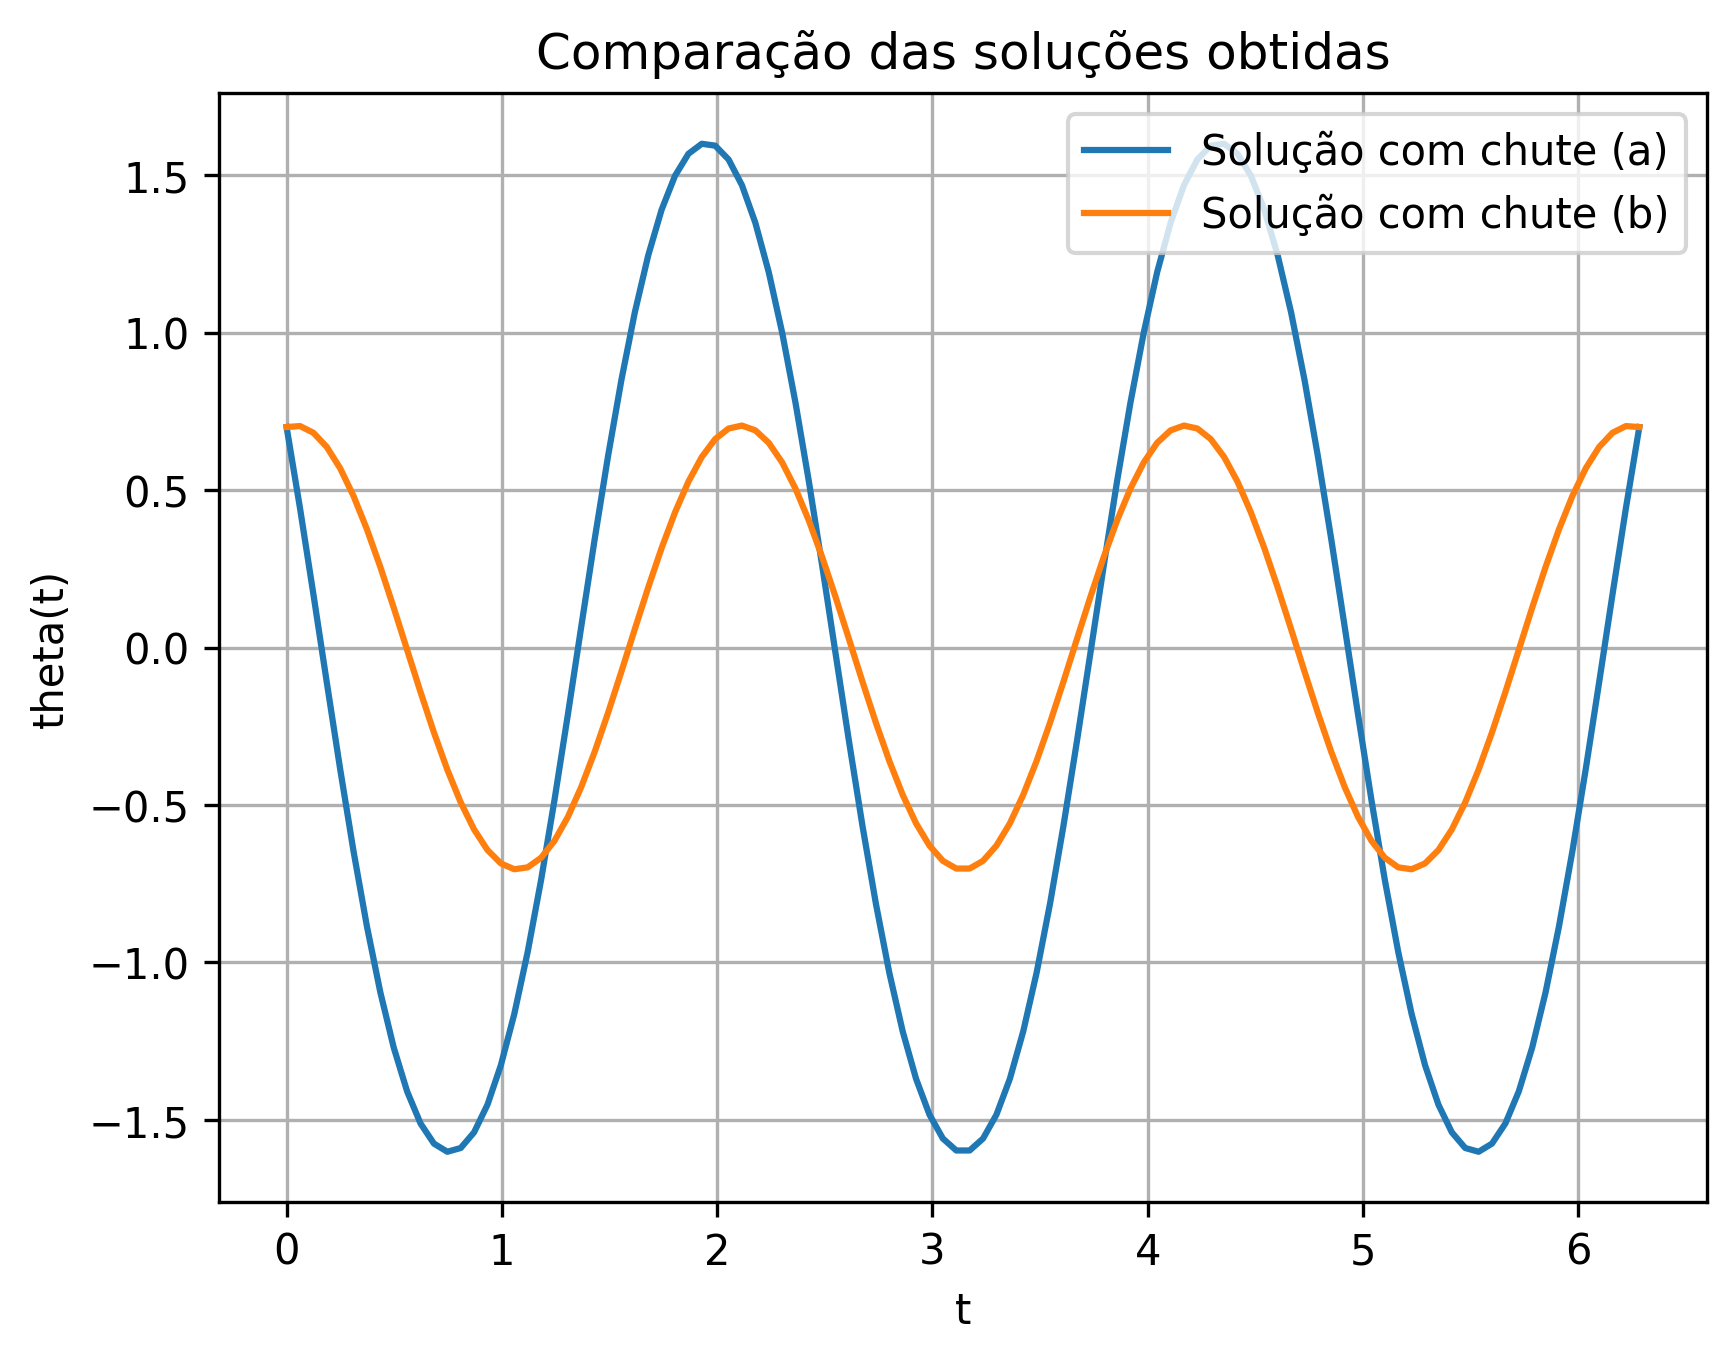
\includegraphics[width=0.7\linewidth]{images/graphics/comparacao_solucoes.png}
        \label{fig:comp-solucoes}
    \end{figure}
\end{frame}

\begin{frame}{Chutes Iniciais}
    \begin{figure}
        \centering
        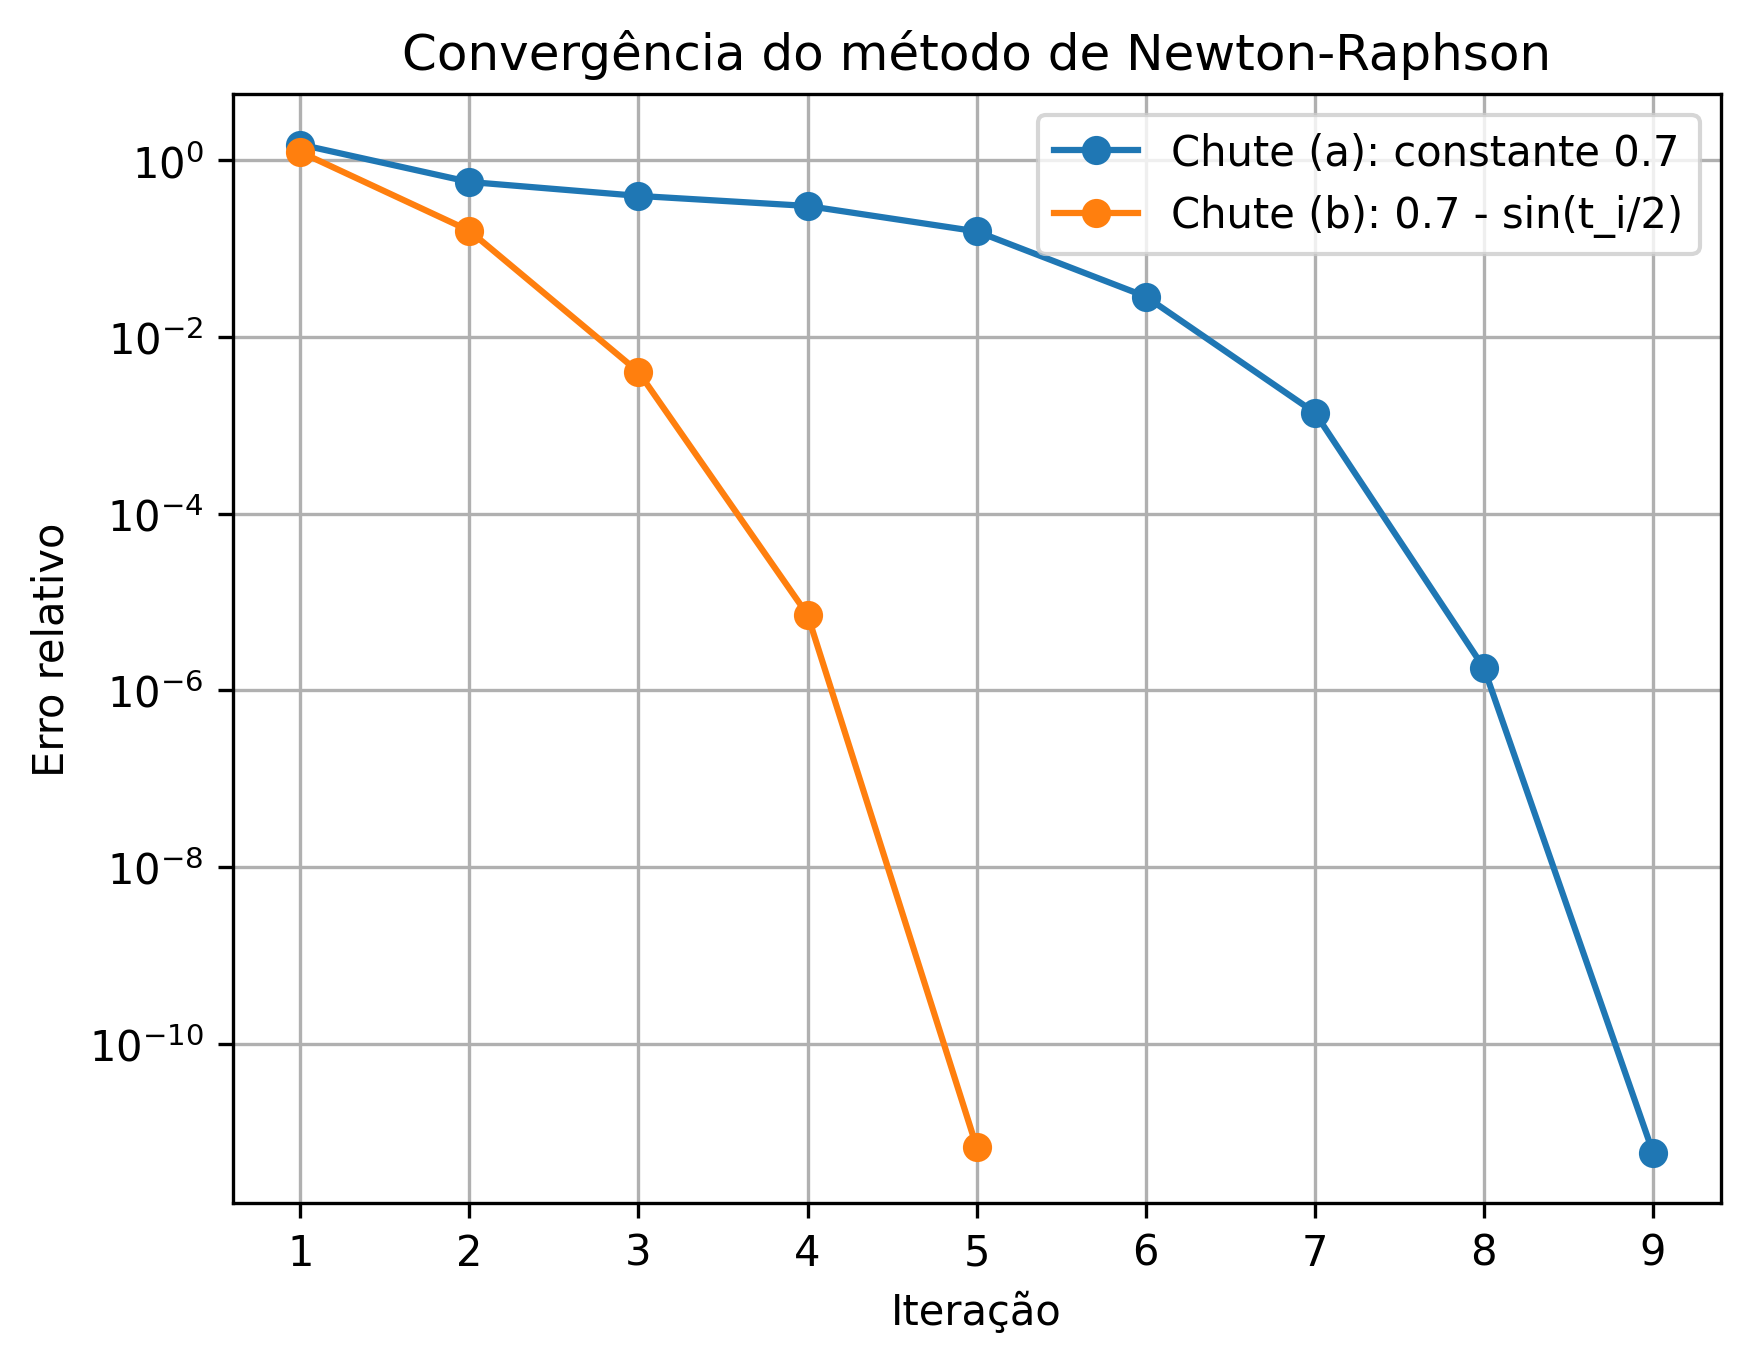
\includegraphics[width=0.7\linewidth]{images/graphics/erro_convergencia.png}
        \label{fig:comp-solucoes-erro}
    \end{figure}
\end{frame}

\subsection{Comparação do uso de Linearização}

\begin{frame}{Linearização}
    \begin{figure}
        \centering
        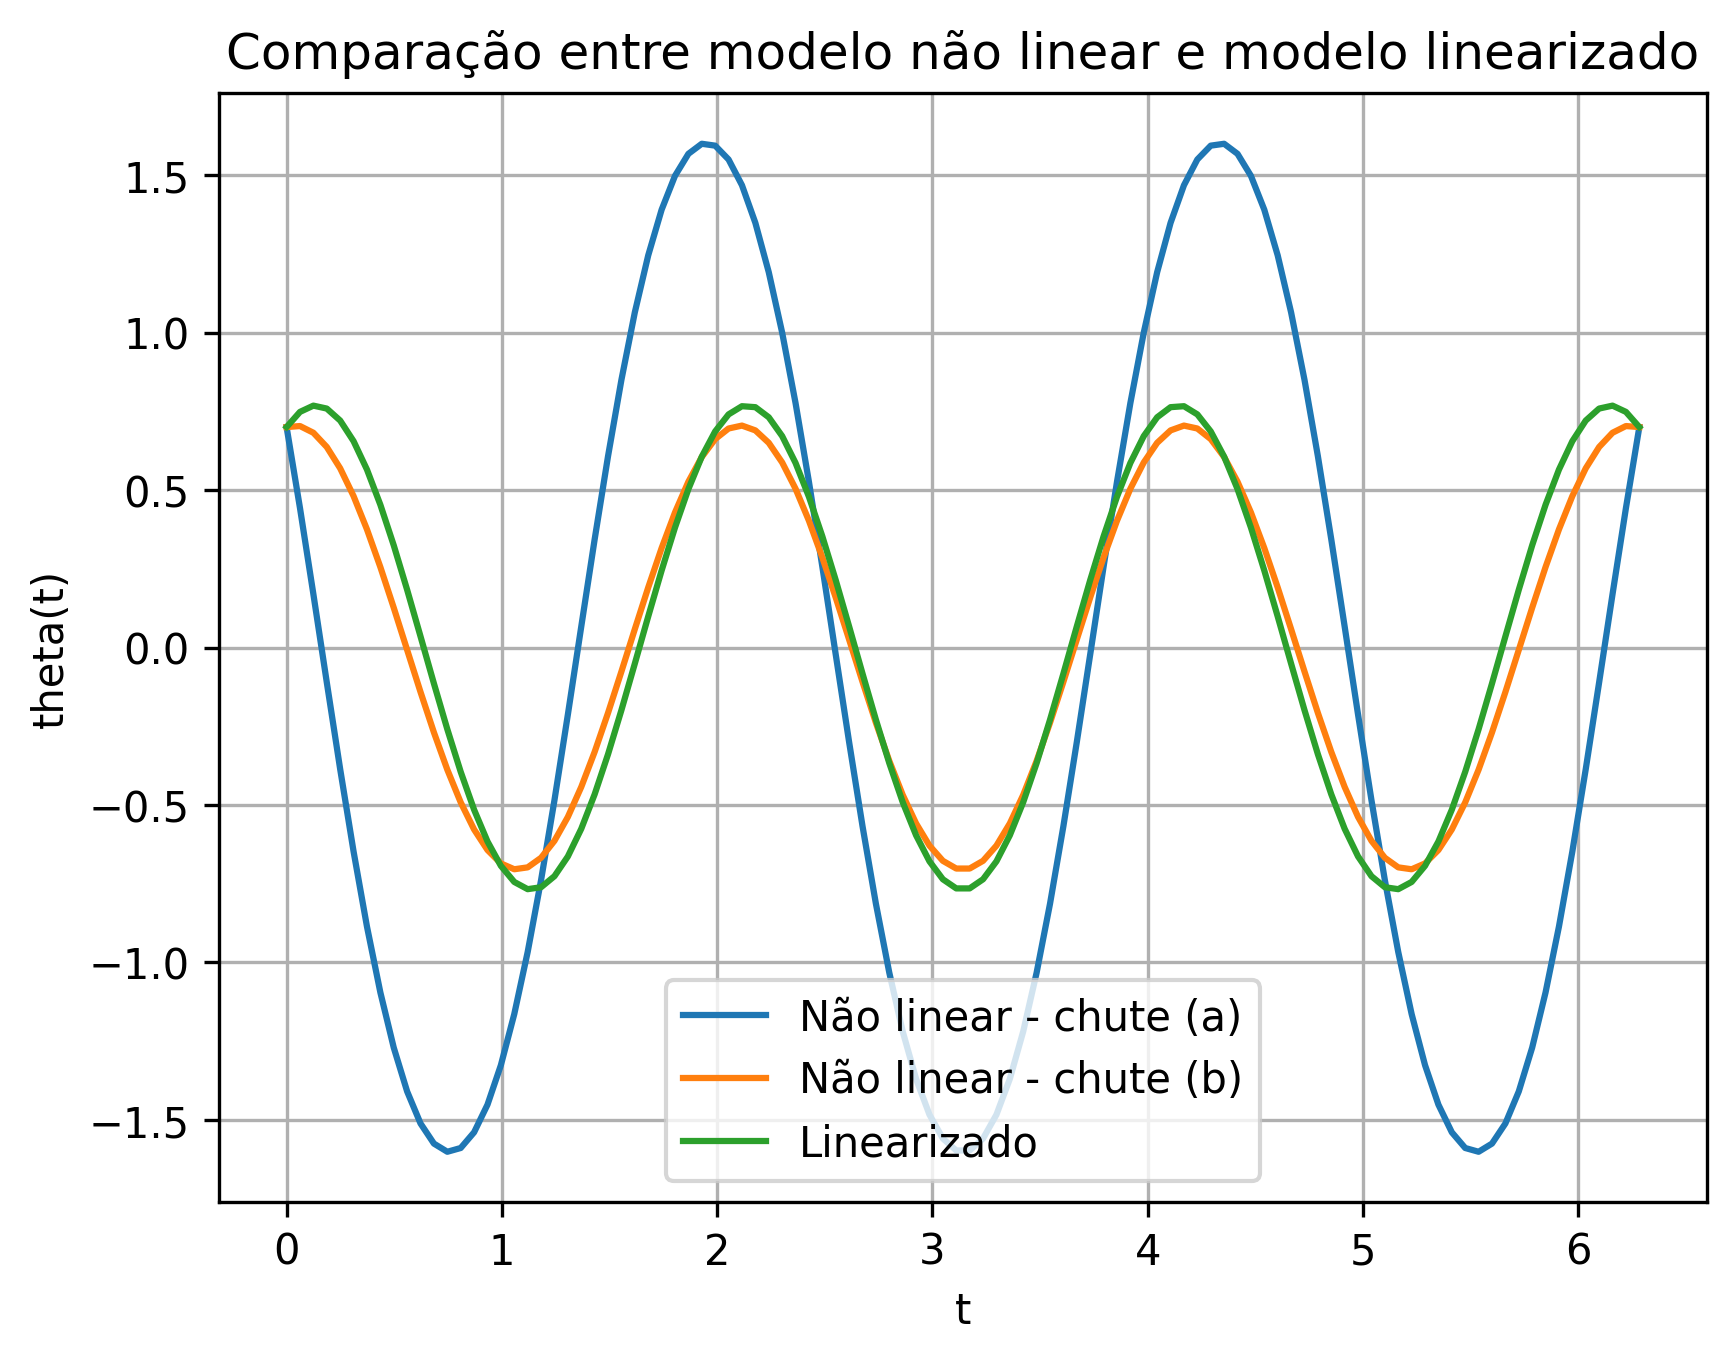
\includegraphics[width=0.8\linewidth]{images/graphics/comparacao_linearizado.png}
        \label{fig:comp-linearizado}
    \end{figure}
\end{frame}

\subsection{Sensibilidade a Alteração de Parâmetros}

\begin{frame}{Alterando Comprimento da Corda}
    \begin{figure}
        \centering
        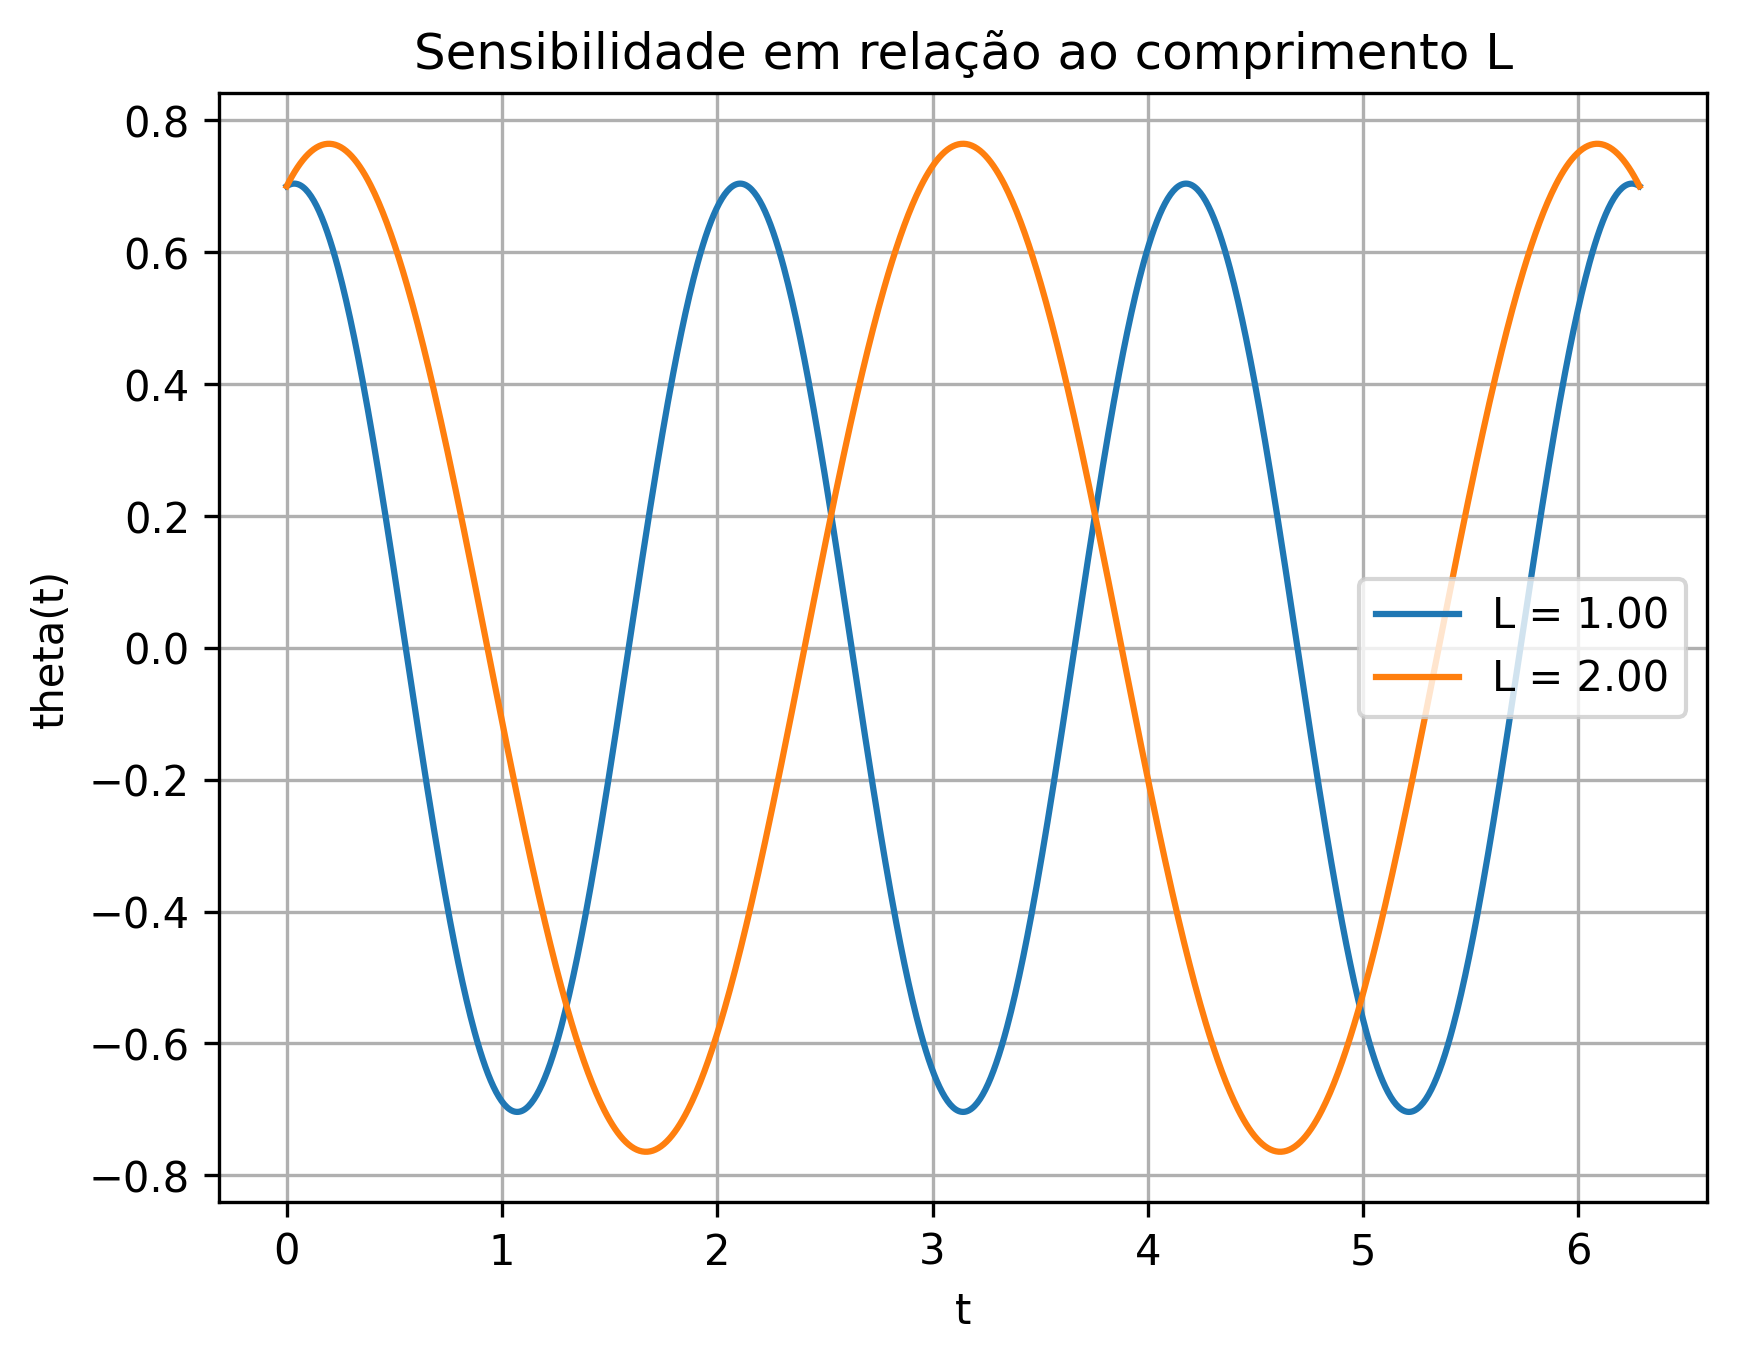
\includegraphics[width=0.8\linewidth]{images/graphics/sensibilidade_L.png}
        \label{fig:alt-L}
    \end{figure}
\end{frame}

\begin{frame}{Alterando Gravidade}
    \begin{figure}
        \centering
        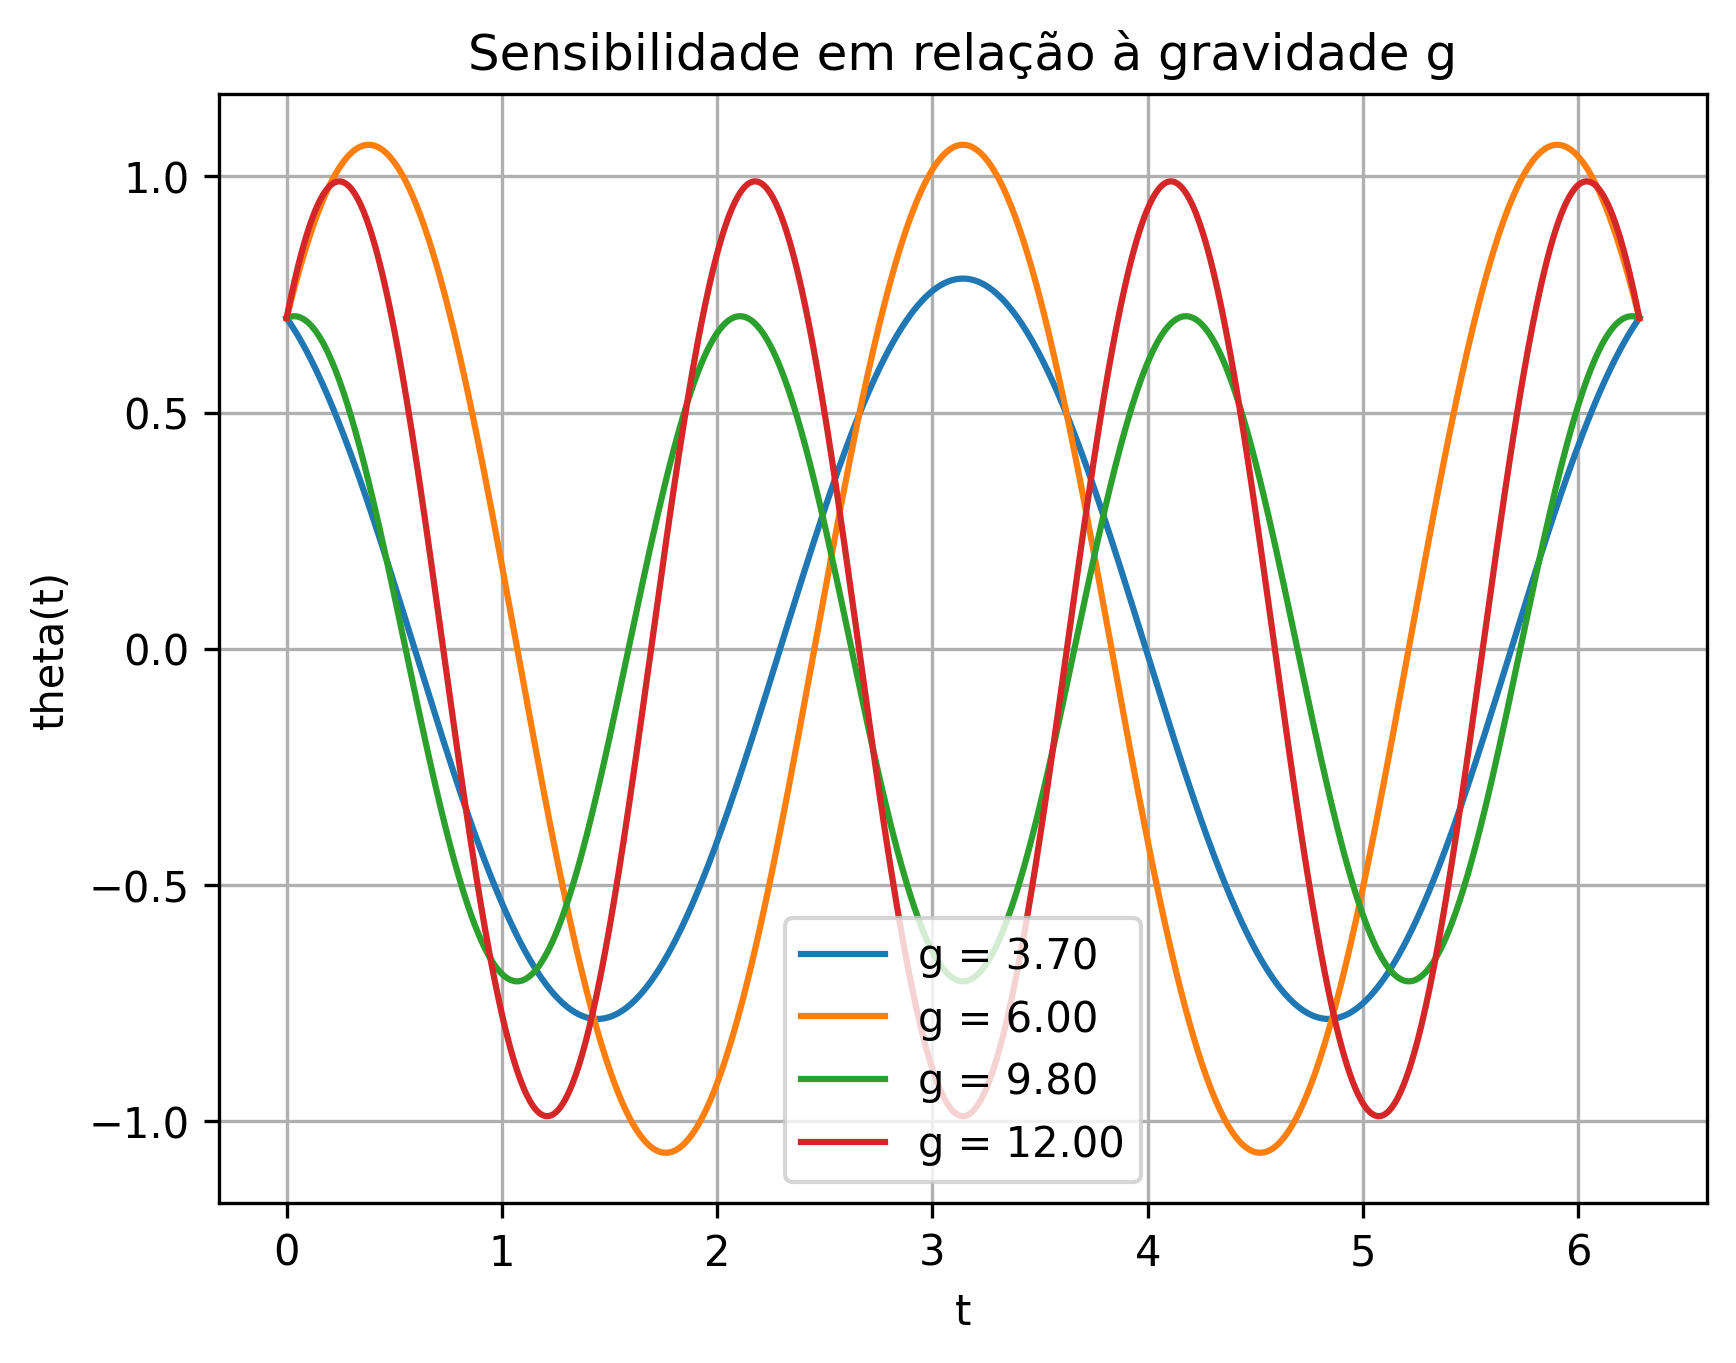
\includegraphics[width=0.8\linewidth]{images/graphics/sensibilidade_g.png}
        \label{fig:alt-g}
    \end{figure}
\end{frame}

\begin{frame}{Alterando Condições Iniciais}
    \begin{figure}
        \centering
        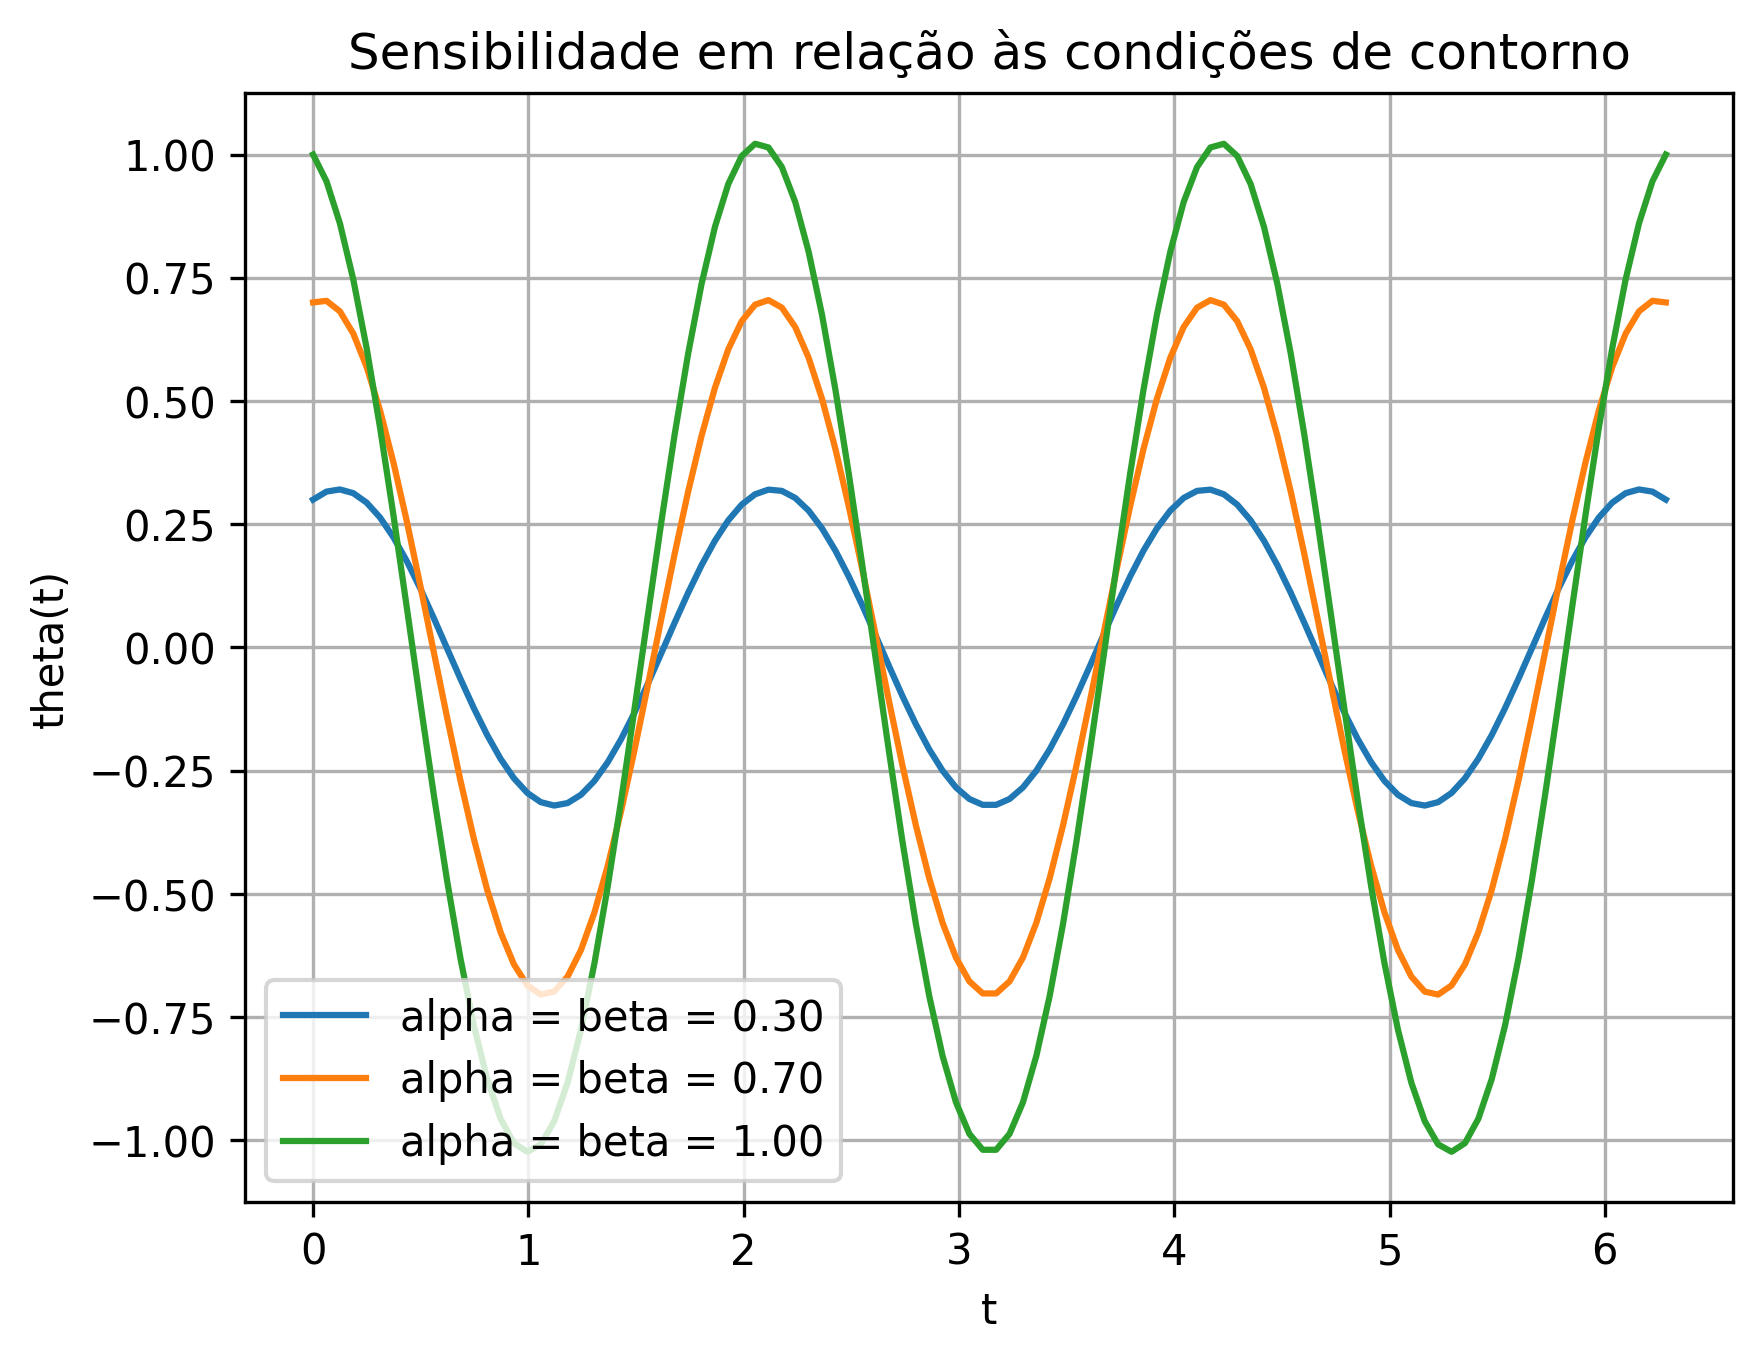
\includegraphics[width=0.8\linewidth]{images/graphics/sensibilidade_alpha_beta.png}
        \label{fig:alt-iniciais}
    \end{figure}
\end{frame}

\end{document}
